\section{Architektura systemu}
\label{chat_architektura_systemu}

Architektura systemu opiera się na klasycznym modelu klient-serwer.

Klienci będą uzyskiwali dostęp do usługi czatu za pośrednictwem przeglądarki
internetowej. Łącząc się z podanym adresem (IP lub domeny), na którym połączeń
nasłuchuje serwer, w pierwszej kolejności przeglądarka będzie próbować połączyć
się z nim przy użyciu protokołu http i standardowego portu 80, wysyłając do
niego żądanie metodą GET. Wówczas, serwer będzie zawsze odpowiadał statycznym
plikiem HTML, zawierającym odwołania do skryptów w języku JavaScript (JS) oraz
pozostałej, statycznej treści (np. grafiki czy arkusze stylów CSS). Serwer
będzie odsyłał te pliki do przeglądarki w odpowiedzi na kolejne żądania HTTP
GET, wysyłane w miarę dalszego renderowania pliku HTML. W ten sposób, po stronie
klienta zostanie pobrana i uruchomiona aplikacja internetowa typu Single Page
Application, której interfejs będzie reagował z użytkownikiem oraz ulegał
zmianom wskutek działania skryptów JS, załadowanych na pierwszym etapie
uruchomienia. Po stronie serwera, dostarczaniem treści statycznych będzie
zajmował się daemon HTTP - Nginx.

Gdy tylko skrypty JS wykryją pobranie wszystkich plików składowych aplikacji
z serwera, podjęta zostanie próba nawiązania połączenia z tym serwerem przy
użyciu protokołu WebSocket. Będzie on od tego momentu podstawowym kanałem
komunikacji pomiędzy klientem a serwerem.

Zgodnie ze standardem WebSocketu, zanim zostanie nawiązane właściwe połączenie,
powinno dojść do „uścisku dłoni” (ang. \textit{handshake}) pomiędzy klientem a
serwerem. W związku z tym, pierwsza próba połączenia również zostanie podjęta
przy użyciu protokołu http, jednakże tym razem pod innym, dedykowanym portem
(w naszym przypadku będzie to port 8000), a także zawierać nagłówki wskazujące
na żądanie zmiany używanego protokołu na WebSocket, jego wersję oraz klucz
(„Sec-WebSocketKey”). Serwer udzieli wówczas odpowiedzi ze swoim własnym
kluczem, informując o zmianie stosowanego protokołu na WebSocket.

W chwili prawidłowego rozpoczęcia połączenia WebSocket, aplikacja po stronie
klienta wyświetli użytkownikowi okno autoryzacyjne. Wpisane tam dane zostaną
następnie przesłane do serwera. Po jego stronie, komunikat zostanie zdekodowany
przez aktora \texttt{WSConnector} i przekazany powiązanemu aktorowi
\texttt{Authorizer}. Jego zadaniem będzie weryfikacja przedstawionych informacji
oraz podjęcie decyzji o autoryzacji lub jej odmowie. Decyzja ta jest odsyłana do
\texttt{WSConnectora} i następnie przekazywana do aplikacji po stronie klienta.

Jezeli autentykacja przebiegnie pomyślnie, aktor \texttt{Authorizer} uruchamia
aktora \texttt{UserSession}, spina go z aktorem \texttt{WSConnector} używanym
wcześniej do komunikacji z frontendem, oraz ulega autodestrukcji.

\newpage

\subsection{Dekompozycja systemu na podsystemy}
\label{architektura_chatu}

\subsubsection{Strona serwera (,,backend'')}
Na serwer czatu składa się grupa współdziałających, ale zupełnie odrębnych od
siebie aktorów, ukazanych na rysunku \ref{diag-komp}

\nameref{diag-komp}.
\begin{figure}[!htp]
	\centering
	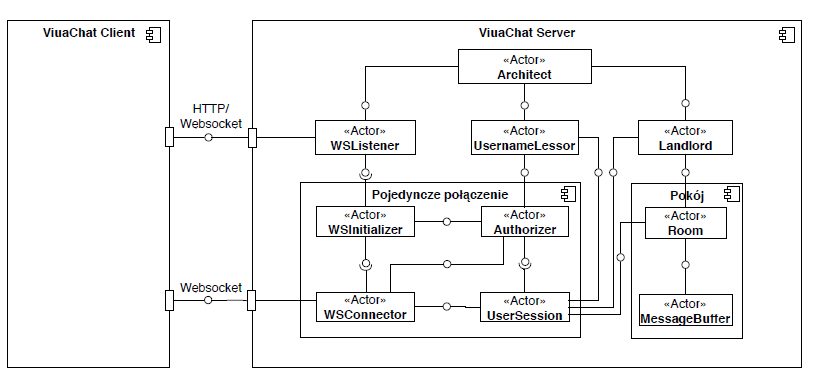
\includegraphics[width=\textwidth]{chat/fig/pck-diag}
	\caption{Diagram komponentów serwera ViuaChat}
	\label{diag-komp}
\end{figure}

\begin{labeling}{UsernameLessor}

  \item[\texttt{Architect}] Uruchamiany jako pierwszy wraz z całym
  serwerem, a następnie inicjalizuje i nadzoruje aktorów \texttt{WSListener},
  \texttt{UsernameLessor} oraz \texttt{Landlord}. W razie nieprawidłwego
  działania lub wyłączenia któregokolwiek z tych trzech głównych aktorów,
  \texttt{Architect} automatycznie zainicjuje przeładowanie całego serwera.
  Ponadto, \texttt{Architect} potrafi w momencie uruchamiania serwera odczytać
  jego pliki konfiguracyjne i na tej podstawie należycie skonfigurować pokoje
  oraz administratorów. Zawsze występuje w jednym egzemplarzu.

  \item[\texttt{WSListener}] Odpowiada za nasłuchiwanie na porcie 8000 po
  stronie serwera, a przy każdej próbie połączenia będzie tworzyć kolejnego,
  niezależnego aktora \texttt{WSInitializer}. Występuje zawsze w jednym
  egzemplarzu.

  \item[\texttt{WSInitializer}] Odpowiada za  realizację ,,uścisku dłoni'' i
  formułowanie odpowiedzi zwrotnej po stronie serwera w odniesieniu do
  połączenia na konkretnym gnieździe. W razie prawidłowego nawiązania
  połączenia, aktor ten utworzy kolejną parę aktorów, \texttt{WSConnector} oraz
  \texttt{Authorizer}, zaś WSInitializer ulegnie samozniszczeniu.

  \item[\texttt{WSConnector}] Odpowiada za dalszą, bezpośrednią obsługę
  przydzielonego gniazda. Występuje ich tylu, ile jest otwartych połącznień.
  Jego rolą będzie również kodowanie i dekodowanie wiadomości (ang.
  ,,messages''), czyli podstawowych logicznych jednostek informacji, które są
  używane przy połączeniach z użyciem protokołu WebSocket. Pilnuje również, czy
  połączenie nie zostało zerwane oraz inicjuje zamykanie sesji użytkownika.

  \item[\texttt{Authorizer}] Wymienia wiadomości od \texttt{WSConnectora}, który
  został uruchomiony wraz z nim i odpowiada za należytą autentykację i/lub
  autoryzację użytkownika w usłudze czatu. Egzemplarz aktora tego typu jest
  powoływany dla każdego otwartego połączenia bez nawiązanej sesji. Aby dokonać
  autoryzacji, aktor \texttt{Authorizer} kontaktuje się \texttt{UsernameLessor}.
  Jeżeli autentykacja przebiegnie pomyślnie, aktor \texttt{Authorizer} uruchamia
  aktora \texttt{UserSession}, spina go z aktorem \texttt{WSConnector} używanym
  wcześniej do komunikacji z frontendem, oraz ulega autodestrukcji.

  \item[\texttt{UsernameLessor}] Jego zadaniem jest zarządzanie informacjami na
  temat tymczasowych nazw użytkowników, należących do	użytkowników bez stałych
  kont (ich gromadzenie, udzielanie, weryfikacja, dbanie o unikalność), a także
  weryfikacja tożsamości kont administratorów z dodatkowym użyciem hasła.
  Występuje w jednym egzemplarzu, przez cały czas istnienia serwera. Ponadto,
  nadzoruje działanie aktorów \texttt{Authorizer} oraz \texttt{UserSession}.

  \item[\texttt{UserSession}] Przejmuje komunikację z użyciem
  \texttt{WSConnector}, pozwalając na zwyczajne użytkowanie czatu. Aktor
  ,,UserSession'' gromadzi informacje na temat nazwy oraz poziomu uprawnień
  użytkownika, a także tego, z jakim pokojem jest obecnie spięty.

  \item[\texttt{Landlord}] Jego zadaniem jest współudział w podpinaniu
  użytkowników do pokoju, tworzeniem nowych i usuwaniem istniejących pokojów, a
  także utrzymywanie i udostępnianie kompletnej listy aktywnych pokojów.

  \item[\texttt{Room}] Działa jak router wiadomości i przechowuje listę użytkowników którzy są do niego wpięci. Istnieje w tylu egzemplarzach, ile jest aktywnych pokojów.

  \item[\texttt{MessageCache}] Przechowuje i odtwarza 10 najnowszych wiadomości wysłanych do pokoju. Występuje po jednym egzemplarzu dla każdego aktywnego aktora \texttt{Room}.

\end{labeling}

\subsubsection{Warstwa interfejsu użytkownika (,,frontend'')}
Podczas pracy nad wartwą frontendu, zastosowano framework webowy Vue.js. Jedną
z przyczyn dla tej decyzji jest możliwość zdekomponowania projektowanej aplikacji na mniejsze części, nazywane modułami (ang. \textit{modules}). Są one zorganizowane hierarchiczne. Każdy z modułów zawiera własny skrypt JavaScript, a także kod HTML i arkusz CSS. Powoduje to, że każdy z modułów jest niezależny od pozostałych i może realizować swoje zadania w pełni autonomicznie.

Każdy z modułów udostępnia swojemu rodzicowi pewne określone parametry. Ich zmiana
jest podstawowym sposobem na interakcję pomiędzy nimi, co jest zgodne z
paradygmatem \textit{data driven application} (z ang. ,,aplikacja sterowana
poprzez dane''). W podobny sposób następuje zmiana kodu HTML modułów. Zamiast
zmieniać węzły DOM w sposób jawny poprzez skrypt, programista wskazuje w
szablonie HTML te miejsca, które ulegają określonym przemianom wraz ze zmianą
wewnętrznych parametrów modułu.

W projekcie przewidziano zastosowanie modułów, przedstawionych na \ref{diag-komp-front}.

\nameref{diag-komp-front}.
\begin{figure}[!htp]
	\centering
	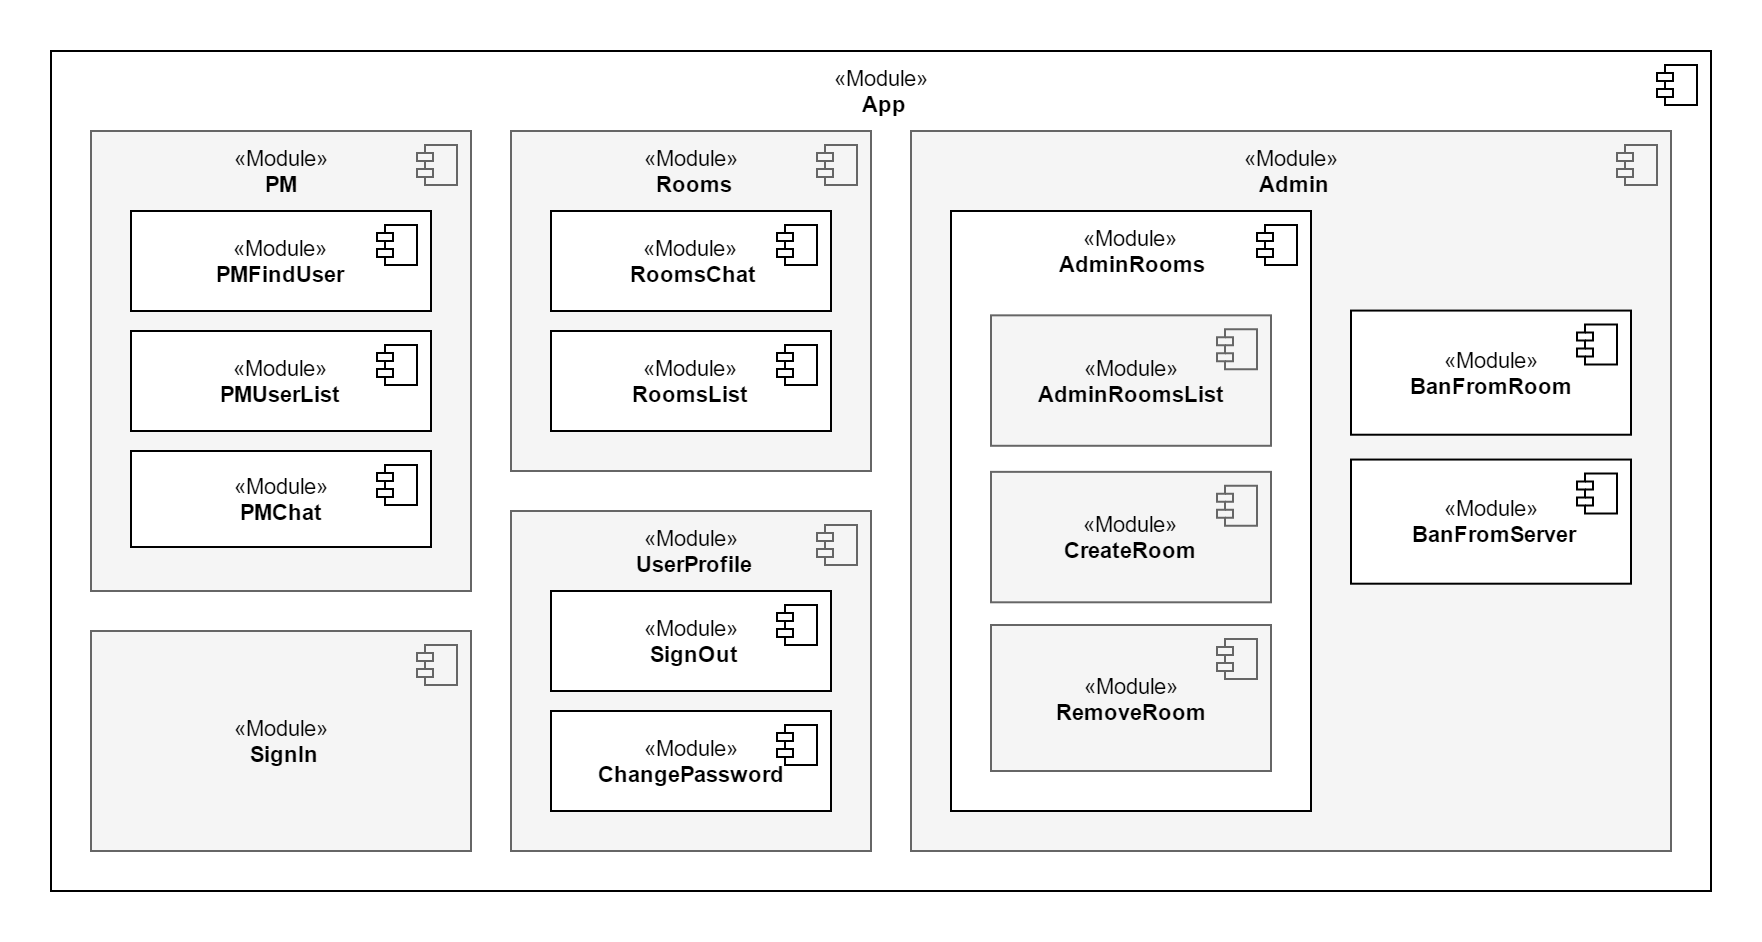
\includegraphics[width=\textwidth]{chat/fig/pck-diag-front}
	\caption{Diagram komponentów aplikacji webowej ViuaChat}
	\label{diag-komp-front}
\end{figure}


\section{Decyzje projektowe}

\subsection{Środowisko docelowe}

\subsection{Środowisko implementacji}

\subsection{Priorytety implementacyjne}

\section{Projekt algorytmów i przyjętych protokołów}

\subsection{Protokół frontend-backend}
Komunikacja pomiędzy frontendem a backendem...

\section{Projekt rozwiązań sprzętowych}

\section{Projekt interfejsu}

\subsection{Interfejs użytkownika}

\subsubsection{Założenia konstrukcji interfejsu}

\section{Projekt bazy danych}

\section{Opis implementacji}
